\subsection{Ola Compiler Introduction}

The Ola-lang compiler compiles the high-level Ola contract code into OlaAsm assembly code supported by OlaVM. 

The general pipeline process is as follows:

\begin{figure}[!htp]
    \centering
    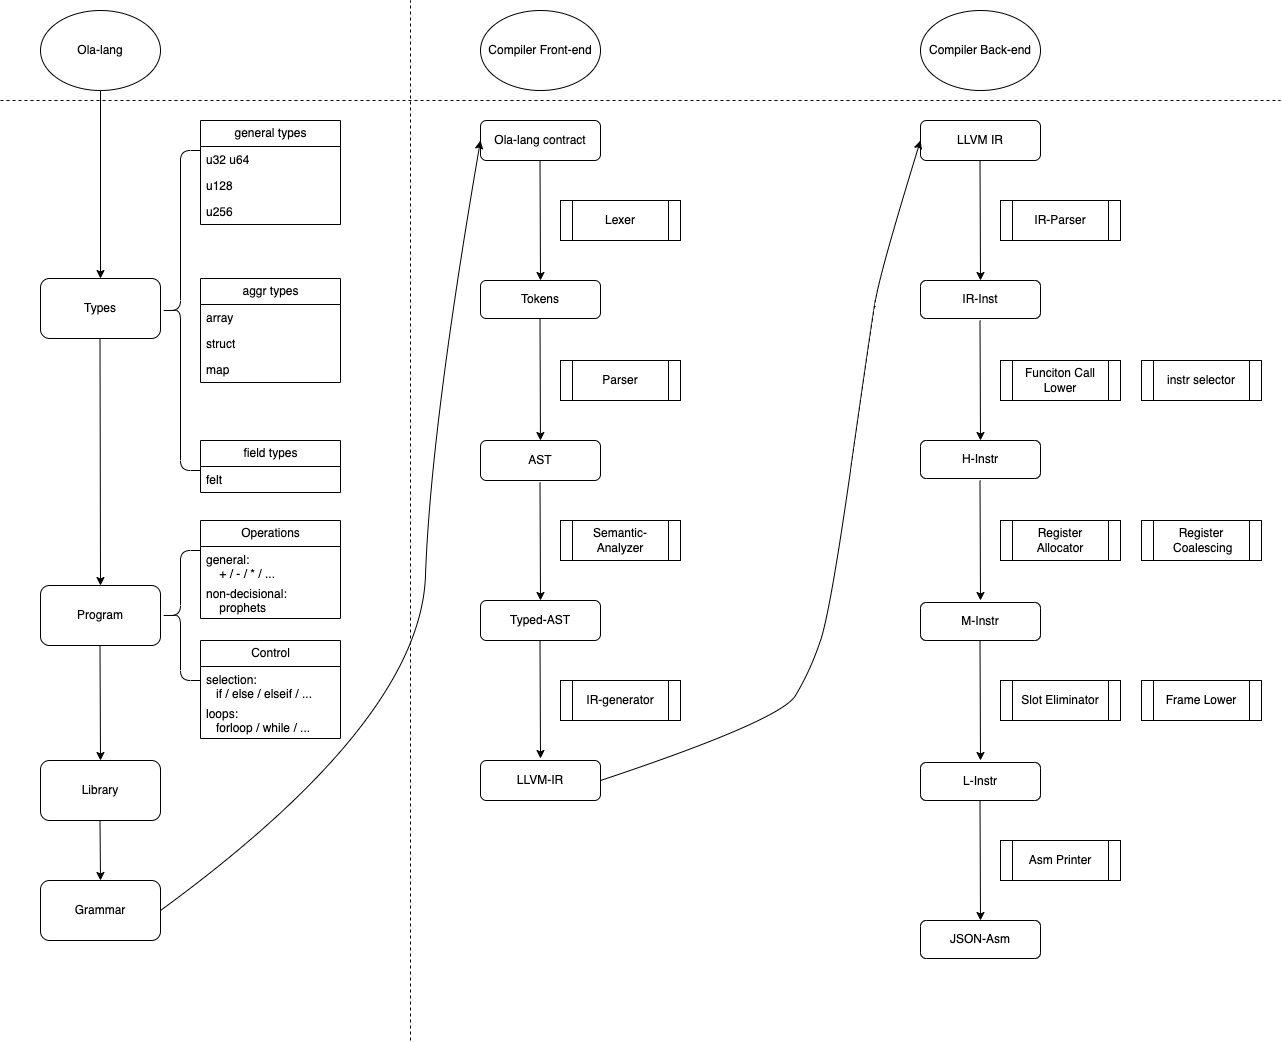
\includegraphics[width=0.6\textwidth]{ola-lang-intro.jpg}
    \caption{Ola-lang pipeline}
    \label{fig:ola-lang-intro}
\end{figure}

As can be seen from the above diagram:

The frontend of the compiler takes the high level contract program as input to compiler it into llvm ir;
and the backend of the compiler takes the llvm ir generated by the frontend as input to compiler it into ola assembly code.

The assembly code is eventually assembled, linked, loaded, and executed by Olavm through the toolchain pipeline to generate trace.


To illustrate the compiler pipeline, the following is an example of a typical u32 type sqrt operation with instructions and prophet two differce versions to show the code generation process.

An example ola-lang high-level language program for computing sqrt of type u32 with prophet version is as follows:
\begin{lstlisting}[language={}]
contract SqrtContract {

    fn main() {
       sqrt_test(4);
    }

    fn sqrt_test(u32 n) -> (u32) {
        u32 b = u32_sqrt(n);
        return b;
    }

}
\end{lstlisting}


An example ola-lang high-level language program for computing sqrt of type u32 with instructions version is as follows:
\begin{lstlisting}[language={}]
contract SqrtContract {

    fn main() {
       sqrt_test(4);
    }

    fn sqrt_test(u32 a) -> (u32) {
        u32 result = 0;
        if (a > 3) {
            result = a;
            u32 x = a / 2 + 1;
            // assume the maximum iteration is 100
            for (u32 i = 0; i < 100; i++) {
                if (x >= result) break;
                result = x;
                x = (a / x + x) / 2;
            }
        } else if (a != 0) {
            result = 1;
        }
        return result;
    }

}
\end{lstlisting}
